\section{Introduction}
\label{sec:introduction}

\begin{figure*}[t]
    \centering
    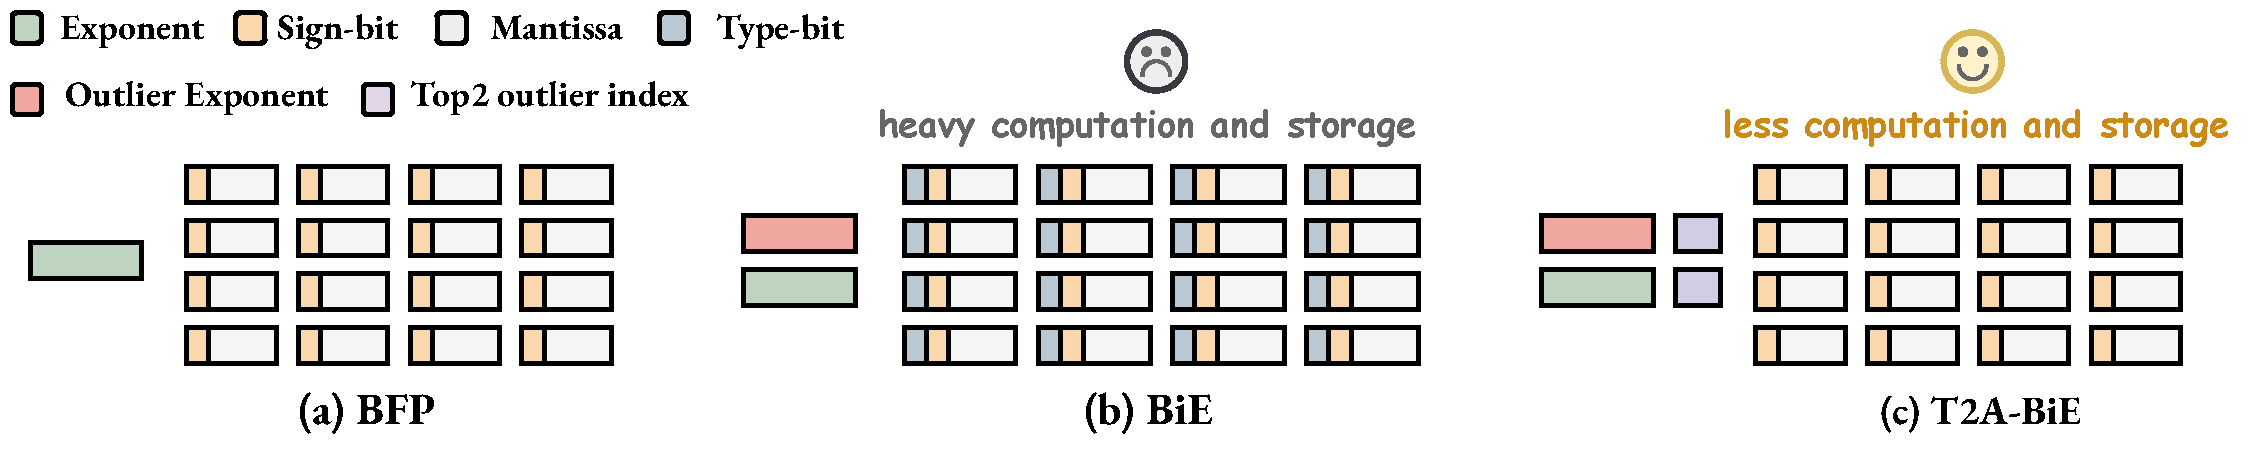
\includegraphics[width=0.95\textwidth]{figures/data-format.pdf}
    \caption{Block-level data formats. (a) Conventional BFP with one shared exponent per block. (b) Bi-exponent BFP (BiE), which adds an outlier exponent and spends a type bit on every element. (c) The proposed Top-2 Activation-only Bi-Exponent BFP (T2A-BiE), which keeps both exponents but replaces the per-element type bits with two outlier indices, so the storage and MAC overhead is lower than that of BiE; weights remain single-exponent BFP as in (a).}
    \label{fig:data_format}

    \vspace{4pt}
    \begin{minipage}[t]{0.48\textwidth}
        \centering
        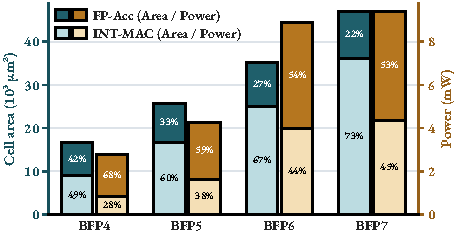
\includegraphics[width=\linewidth]{figures/baseline_bfp_pe_component_power_area.pdf}
        \caption{Component-level power and area of a synthesized baseline BFP-PE (TSMC 90\,nm, 100\,MHz). Power is measured under LLaMA2-7B's real activation distribution.}
        \label{fig:bfp_pe_ppa}
    \end{minipage}%
    \hfill
    \begin{minipage}[t]{0.48\textwidth}
        \centering
        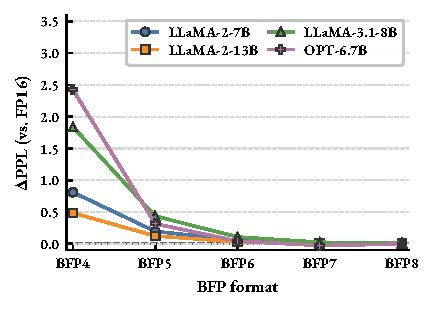
\includegraphics[width=\linewidth]{figures/vanilla_bfp_delta_ppl_g16.pdf}
        \caption{WikiText-2 $\Delta$PPL of vanilla BFP versus FP16 as the mantissa width decreases (group size 16).}
        \label{fig:vanilla_bfp_delta_ppl}
    \end{minipage}
\end{figure*}

Low-precision quantization is essential for deploying large language models (LLMs) under tight memory and energy budgets.
Block Floating Point (BFP) offers a favorable accuracy--cost tradeoff by assigning a shared exponent to each fixed-size block while storing only low-bit mantissas~\cite{msfp2020,fast2022}.
Recent BFP accelerators perform intra-block multiply--accumulate (MAC) with fixed-point arithmetic, but inter-block partial sums with mismatched exponents must still be merged in a floating-point accumulator (FP-Acc)~\cite{bucketgetter2023,winacc2025,smartblock2025,mgs2025}.

Two coupled bottlenecks limit the efficiency of BFP-based LLM inference.
First, the FP-Acc dominates processing-element (PE) cost: in synthesized low-bit configurations it can account for up to 68\% of power and 42\% of area~\cite{bucketgetter2023,winacc2025,smartblock2025}.
Second, activation outliers compress the effective mantissa of co-located normal values and widen the exponent spread of partial sums, increasing FP-Acc activity~\cite{bie2024,oiso2026,bbal2025,harmonia2026}.

This paper develops a hardware-friendly co-design that addresses both bottlenecks jointly.
Our contributions are:
\begin{itemize}
    \item \textbf{Dynamic Exponent-Window Accumulation (DEWA):} a low-cost accumulator that retains partial sums within a sliding exponent window and forwards only out-of-window updates to the FP-Acc.
    \item \textbf{Activation-only bi-exponent encoding with Top-2 selection:} weights remain single-exponent BFP while activations use a bounded bi-exponent format that retains at most two outliers per block, reducing storage and MAC control overhead relative to full BiE~\cite{bie2024,oiso2026}.
    \item \textbf{Evaluation on LLaMA2-7B:} we quantify perplexity, outlier occupancy, and FP-Acc request reduction under a consistent WikiText-2 protocol, showing negligible accuracy loss for the proposed W-BFP4 / T2A-BiE4 design point.
\end{itemize}

The remainder of this paper reviews BFP deployment challenges (Section~\ref{sec:background}), presents DEWA, Top-2 selection, and Hybrid Top-2 DEWA (Section~\ref{sec:design}), describes the Top-2 index encoding and the DEW-based PE datapath (Section~\ref{sec:architecture}), reports experimental results (Section~\ref{sec:evaluation}), and concludes (Section~\ref{sec:conclusion}).
